\subsection{PGC}

PGC \cite{PGC} is a standalone auditable confidential payment system. In this work they trade anonymity for highly efficient auditing only dependent to the number of past user transactions. Privacy is offered in terms of confidentiality and use pseudonymity as a feature assuming that auditors can link the account addresses with real identities. It proposes two kinds of auditing mechanism: (i) regulation compliance that is achieved through three audit functions, namely transaction limits, tax payment and selective value disclosure. (ii) supervision (tracing functionality) that is achieved through including the necessary auxilary information in the transaction structure. The cryptographic techniques that are used for its implementation is a variant of El Gamal encryption and zk-proofs composed of $\Sigma$-protocols.

\subsubsection{Entities}
More specifically, the system consists of the following entities:
\begin{itemize}
    \item Users: Individuals that transact with each other and may control several accounts within the system.

    \item Validators: Validators are responsible for checking the validity of proposed transactions within the system. They ensure that transactions meet the required criteria before being included in the blockchain.
    
    \item Regulators: Regulators interact with involved users to verify if a set of transactions complies with system's policies, without holding any secret information.
    
    \item Supervisors: Supervisors have access to a global trapdoor, which allows them to monitor and trace transactions without interacting with the involved users. 
\end{itemize}

\subsubsection{Accounts}
In order to be able to interact with a system a user creates an account. Each account is associated with a secret key $\sk$, a public key $\pk$, which represent the pseudonym of the user within the system, an encoded balance $\tilde{C}$ , and an incremental serial number $sn$ used to prevent replay attacks ($ \acct = (\sk, \pk, \tilde{C}, sn)$). The balance is encrypted in order privacy to be achieved. Only the owner of $\sk$ can decrypt and learn the value but all users should be able to change the encrypted value. PGC implement this through homomorphic encryption.

\subsubsection{Transactions}
Users can use the accounts to transact within the system. A transaction take place between two participants and need as input the secret key of the sender $\sk$, the transacted value $v$ and the public keys of both sender and receiver ($\pk_s, \pk_r)$. Given the input the algorithm produces $(C_s, C_r)$ that are encoded transferred value $v$ under the public keys of sender and receiver $(\pk_s, \pk_r)$.

The legality of the transaction is proved through the creation of a a zk-proof $\pi_{legal}$. $\pi_{legal}$ consists of the following proofs: (i) $\pi_{equal}$: $C_s, C_r$ contains encryption of the same value $v$ (ii) $\pi_{right}$: the transfer amount $v$ is within the allowed limits (iii) $\pi_{solvent}$: the sender has enough balance.

Finally, to authenticate that the sender is the owner of the corresponding account the algorithm sign the $(sn, memo = (\pk_s, \pk_r, C_s, C_r), \pi_{legal})$ with the secret key $\sk$ producing the signature $\sigma$.

The final transaction is $\txn = (sn, memo, \pi_{legal}, \sigma)$.

In order to support supervision under a specified authority with a known public key $\pk_a$ the transaction can be extended with an encryption of transacted value $C_a$ under the $\pk_a$. Then the supervisor can inspect any confidential transaction by decrypting $C_a$ using $\sk_a$.

\begin{figure}[h]
    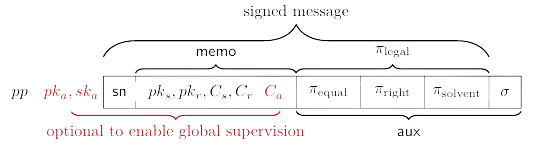
\includegraphics[width=\textwidth]{images/pgc/pgc_txn.png}
    \centering
    \caption{Data structure of transaction in PGC}
\end{figure}


\subsubsection{Policies and Audit}
In PGC policies are represented as predicates $f$ over a public key $\pk$ and related transactions $\{\txn_i\}_{i=1}^n$ in which $\pk$ participates either as sender or as receiver. Let $v_i$ the transferred amount in $\txn_i$. They implement the following policies over the values $v_i$:
\begin{itemize}
    \item Limit policy $f_{limit}(\pk, \{\txn\}_{i=1}^n)$: Checks that $\sum_i^n {v_i} \leq a_{max}$, where $a_{max}$ is an upper bound depending on application. The prover can be either the sender or the receiver of $\txn$. This policy is a mechanism used for anti-laundering money.
    \item Tax policy $f_{tax}(\pk, \txn_1, \txn_2)$: Let $\pk$ be recipient in $\txn_1$ and sender in $\txn_2$. Let $v_1,v_2$ be the transfer amounts in each transaction. The policy checks if $v_1/v_2 = \rho$, where $\rho$ is a rate depending on application. The auditor can use this policy to ensure that user paid appropriate tax.   
    \item Open policy $f_{open}(\pk, \txn)$: Checks that the underlying transferred amount $v$ is equal to a $v^*$ ($v=v^*$), where $v^*$ is an application-dependent value. The prover can be either the sender or the receiver of $\txn$. The auditor can use this policy to enforce selective-disclosure.
\end{itemize}

\begin{figure}[h]
    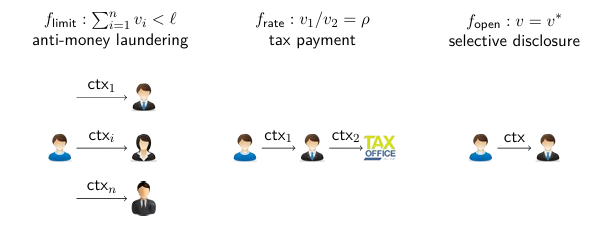
\includegraphics[width=\textwidth]{images/pgc/pgc_policies.png}
    \centering
    \caption{Policies in PGC}
\end{figure}


In order the auditing to be efficient in PGC it is executed with the aid from the auditee. In particular, it needs the consent of the auditee who creates a zk-proof that proves that they are compliant with the specified policy. The zk-proofs are implemented by using bulletproofs and $\Sigma$-protocols.

% \subsubsection{Implementation}
% As mentioned PGC is composed of a homomorphic encryption scheme, a signature scheme and zk-proofs. In order to implement the first an ISE (Integrated Signature and Encryption) scheme is used. This ISE scheme is instantiated by combining a version of El Gamal encryption, Twisted El Gamal \autoref{TwistedElGamal}, and Schnorr signatures \autoref{Schnorr}, due to the fact that this two cryptographic primitives share the same $\setup, \kgen$ algorithms.In \cite{PGC} it is proved that the obtained ISE scheme is jointly secure if the the twisted ElGamal is IND-CPA secure and the Schnorr signature is EUF-CMA secure.

% Using this implementation the NIZK protocol for the proof system can be created for the validity of the transactions and for the system policies.

% As mentioned in the transactions, $L_{legal}$ can be decomposed in $L_{equal} \land L_{right} \land L_{open}$. 
% \begin{itemize}
%     \item \textbf{NIZK for $L_{equal}$}:\\
%         According to implementation $L_{equal}$ can be written as:
%         \begin{equation*}
%             \{(\pk_1, X_1, Y_1, \pk_2, X_2, Y_2) | \exists r, v \text{ s.t. } X_i = \pk_i^{r} \land Y_i = g^{r} h^v \text{ for } i=1,2 \}
%         \end{equation*}
%         In Twisted ElGamal the randomness $r$ can be safely reused in the 1-plaintext/2-recipient setting. % //TODO: prove this in the crypto section

%         \textbf{$\Sigma$-protocol $\Sigma_{equal}$}:
%         \begin{center}
%             \begin{tabular}{ |l c l| }
%              \hline
%              & ($\pk_1, \pk_2, X_1, X_2, Y$) & \\   
%              \textbf{Prover}($r,v$) &  & \textbf{Verifier} \\
%              $a,b \sample \mathbb{Z}_p$ & & \\
%              $A_1 \gets \pk_1^a, A_2 \gets \pk_2^a$ & $\xlongrightarrow{A,B}$ & \\ 
%              & $\xlongleftarrow{e}$ & $e \sample \mathbb{Z}_p$ \\
%              $z_1 \leftarrow er+a$ &  & \\
%              $z_2 \leftarrow ev+b$ & $\xlongrightarrow{z_1, z_2}$ & Check\\
%              & & $\pk^{z_1} =  AX^e$ \\
%              & & $g^{z_1} h^{z_2} = BY^e$ \\  
%              \hline
%             \end{tabular}
%         \end{center}
%     \item \textbf{NIZK for $L_{right}$}
%     \item \textbf{NIZK for $L_{open}$}
% \end{itemize}

\subsubsection{Setback}
Although PGC does not suffer from the scalability issues of zkLedger, it is not fully private. As mentioned before, PGC offers only confidentiality when it comes to privacy and trades anonymity in order to implement efficient auditability.